\section{Maintenance plan}

In the previous section, we explained a number of basic view expressions 
(selection, projection, join, etc.) that our system can materialize and 
update incrementally, as base data changes. However, queries for data 
analysis are usually a lot more complex. They consist of multiple, 
nested view expressions; these can be applied in any order to build 
higher level constructs. The following query $q$ combines a selection 
and a sum aggregation on a table $A$: 


\begin{center} Select Sum($c_2$) From $A$ Group By $c_1$ Where $c_2 < 10$\end{center} 


In order to build a \textit{maintenance plan}, we decompose the given 
query into a number of basics view expressions. These basic view 
expressions are connected with each other. They form a chain that 
computes and maintains the result of the query. In the chain, each view 
expression computes an intermediate result; which is materialized into a 
view table and the updates on this view table are passed to the next 
view expression. This way, each single base operation propagates along 
the maintenance chain. The last materialized view in the chain 
represents the final result of the query. 





\begin{figure}[h!] 
	\centering 
	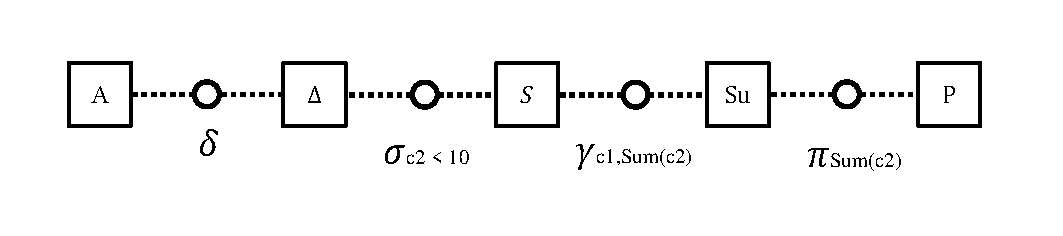
\includegraphics[width=\linewidth]{figures/MaintenanceExample}  
	\caption{Maintenance plan} 
	\label{fig:maintenance_plan} 
\end{figure} 



 Figure~\ref{fig:maintenance_plan} shows the maintenance plan of query 
$q$. A maintenance plan always comprises a set of materialized tables 
(i.e. base tables and view tables), which 
Figure~\ref{fig:maintenance_plan} depicts as boxes; as well as a set of 
view expressions, which Figure~\ref{fig:maintenance_plan} depicts as 
small circles. The dotted lines represent the paths, along which the 
view updates flow to update the whole chain. 

On the very left side of the figure, the base table $A$ -- over which 
$q$ is defined -- is shown. The base table is always the starting point 
of the maintenance chain. In case of a join operation, there can be 
multiple base tables. In example of $q$, the query is just defined over 
one base table $A$. To the right side of base table $A$, a delta 
expression (i.e. $\delta$) follows to build the intermediate view table 
$\Delta$. The connection between $A$ and $\Delta$ implies the following: 
all client operations that are applied to base table $A$, are modified 
by the $\delta$ expression (i.e. their delta is evaluated) and stored to 
the $\Delta$ view. Next to the $\Delta$ view, a selection expression 
(i.e. $\sigma$) build a connection to the intermediate view $S$. The 
$\sigma$ expression drops or passes (based on the selection criterion) 
the client operations from $\Delta$ to $S$. In the next to steps, a sum 
aggregation ($\gamma$) and a projection expression (i.e. $\pi$) succeed 
$S$ to complete the maintenance chain. Expression $\pi$ represents the 
last expression such that view $P$ holds the final result of the query. 




\begin{figure*} \centering 
	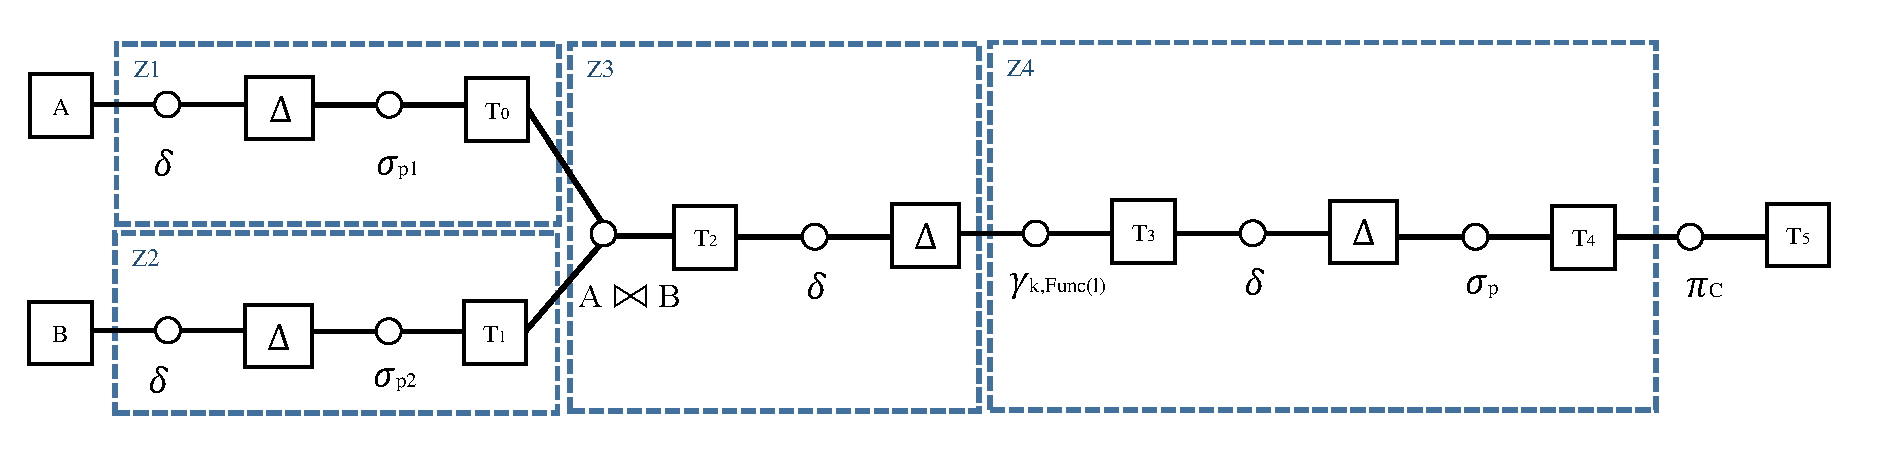
\includegraphics[width=\linewidth]{figures/SQLPattern} 
	\caption{SQL pattern} \label{fig:sql_pattern} 
\end{figure*} 





\subsection{DAG}

In order to describe a maintenance plan for a SQL-query (e.g. the plan 
in Figure~\ref{fig:maintenance_plan}), we use a so-called AND-OR-DAG 
(reference). The AND-OR-DAG was developed in the context of query 
optimizing. Since it is a perfect fit for our needs, we adapt the 
concept to describe and optimize the maintenance in our VMS. Every 
SQL-query has a corresponding maintenance plan, which can be described 
by a AND-OR-DAG. As the name says, the AND-OR-DAG is a directed acyclic 
graph. It alternates between view tables and view expressions; We denote 
the maintenance plan as $P=(V,E)$, where $V$ is a set of 
vertices and $E$ a set of edges. A vertex $v \in V$ is either a table 
vertex $V_T$ with $T=T_0,..T_n$ and or an expression vertex $V_X$ with 
$X=\{\delta, \sigma, \gamma, etc..\}$ . An edge $e \in E$ either 
connects a table vertex and an operation vertex or two expression 
vertices (concatenation). 


 Each query can be translated into a maintenance plan $p \in P$. 
 For example, the query $q$ from Figure~\ref{fig:maintenance_plan} 
 translates to a plan $p$ where $V=\{A, \delta, T_0, \sigma, 
T_1, \gamma, T_2, \pi, T_3\}$ and $E=\{A\rightarrow\delta, 
\delta\rightarrow T_0,...T_2\rightarrow\pi, \pi\rightarrow T_3\}$. 
Through changing the order of operations or combining multiple view 
tables (i.e. executing different optimization), new maintenance plans
can be constructed. These plans represent distinct DAGs, but they 
all compute the same result. We capture those maintenance plans in a set
 $P_q=\{p_1,....p_n\}$. 




\subsection{Translation of SQL pattern} 

So far, we have shown how we a maintenance plan can be derived for a 
single query $q$. As we strive for supporting full SQL semantics, we now 
explain how a complete \textit{SQL pattern} can be translated into a 
maintenance plan. This pattern is a blueprint to translate any type of 
SQL query. Though, the pattern can also be applied to describe nested 
SQL queries, we only discuss simple SQL queries (i.e. every view 
expression only occurs once). A usual SQL parser evaluates the clauses 
of a simple SQL query in the following order: from, where, group by, 
having, select, order by. We use these clauses and translate them into a 
general maintenance pattern (AND-OR-DAG). By removing elements that are 
not part of a query, every other simple query can be constructed. 

As a first step, we map the clauses of a SQL query to the respective 
basic view expressions: from translates to one (or in case of a join) 
multiple base tables; the where clause translates to a Selection 
expression ($\sigma$); the group by translates to an aggregation (sum, 
count, min, max, depending on the aggregation function) expression; the 
having clause is just another selection expression; and, finally, the 
select clause translates to a projection expression. 

Figure~\ref{fig:sql_pattern} shows the generalized maintenance plan of a 
simple SQL query. As before the figure depicts table vertices as boxes 
and expression vertices as small circles. The dotted areas are 
\textit{zones}. The table vertices in a zone share the same row key 
(i.e. primary keys of the tables). This is insofar of interest as view 
tables within a zone can be merged to share the results of multiple view 
expressions at once. We will use this property later in the paper to 
reduce the amount of intermediate view tables. 

On the very left side of Figure~\ref{fig:sql_pattern} you can see two 
base tables $A$ and $B$. Both base tables are followed by a delta 
expression and the respective view table, as the changes in both tables 
need to be tracked. In the next step both delta tables are connected to 
a selection expression ($\sigma$) with different predicates ($p_1$ and 
$p_2$). Selection expressions (i.e. where clauses) are usually evaluated 
first in SQL queries; they are defined over a base tables only and they 
can reduce the amount of operations, passed to subsequent views, 
significantly. Applying a selection to a record doesn't change the row 
key. That is why $\Delta$ and Selection views are located in the same 
zone. 

 View tables $T_0$ and $T_1$ are combined to $T_2$ by a join expression. 
A join is usually evaluated in the from clause of a query. In 
Figure~\ref{fig:sql_pattern}, two base tables $A$ and $B$ are joined. In 
general, the from clause of a query could contain a join on $n$-tables. 
For that case, we distinguish two cases: (1) All base tables are joined 
on the same join key. (2) Different pairs of join tables are joined on 
different join keys. Case (1) is trivial, as we still obtain one join 
view and one join expression with $n$ input edges from the different 
delta tables. In case (2), we have to build a join view for each join 
pair and combine those join views again until just one join view 
remains. 

After a join expression, the row key changes. There are joins (e.g. 
key/foreign-key) where the row key of one of the join tables can be 
used. However, as we control the process of view maintenance and we aim 
at generality, the row key of a join table is always the composite key 
of both base tables. Therefore, the join table $T_2$ also defines a new 
zone. A table in a new zone has to be followed by another $\Delta$ view 
to, again, track the changes of its records. At a first glance, the high 
amount of delta views may appears like a big overhead in the system; but 
during the optimization phase this overhead nearly vanishes, as most of 
the delta views can be combined with other expressions and don't need to 
be materialized separately. 

After the second $\Delta$ view, an aggregation expression (e.g. a sum 
view) is applied to the maintenance plan. It is what we need when a 
group by clause in a query defines a set of aggregation keys and the 
select statement defines a set of aggregation functions and their 
respective values. Thus the aggregation view is, in general, defined as 
$\gamma A,Func(X)$. Like the join view, the aggregation expression 
enforces another row key in view $T_3$. Again, there are special cases, 
where the join key might be equal to the aggregation key. But as we aim 
at generality, we assume that the aggregation expression starts a new 
zone (i.e. $Z_4$). As before, the change of row keys in $T_3$ is 
followed by a delta expression. The last view expression in $Z_4$ is 
another selection ($\sigma p$). It is derived from the optional having 
clause in a SQL query. This selection is treated exactly like the first 
selection, just that it operates upon the records of an aggregation and 
not of a base table. 

The last view expression, the projection ($\pi C$) is present in most 
of the queries, as it is mapped from the select clause in a query. The 
projection doesn't necessarily has to be the last expression of the 
maintenance plan. It can also be materialized earlier. The projection 
only influences the number of columns. Thus, the resulting view uses 
whatever row key is taken in the preceding view. That is also the reason 
why view $T_5$ is not located within a special zone. 

Now, we have mapped all possible query clauses (except the sort clause),
building a maintenance plan from a query is straight forward. If a clause
exists in the query the according view expression and its materialized
result are added to the graph. The order, in which the vertices are added
to the maintenance plan, is depicted in Figure~\ref{fig:maintenance_plan}.
The maintenance plan that belongs to a query is also called query DAG.

\begin{figure} \centering 
	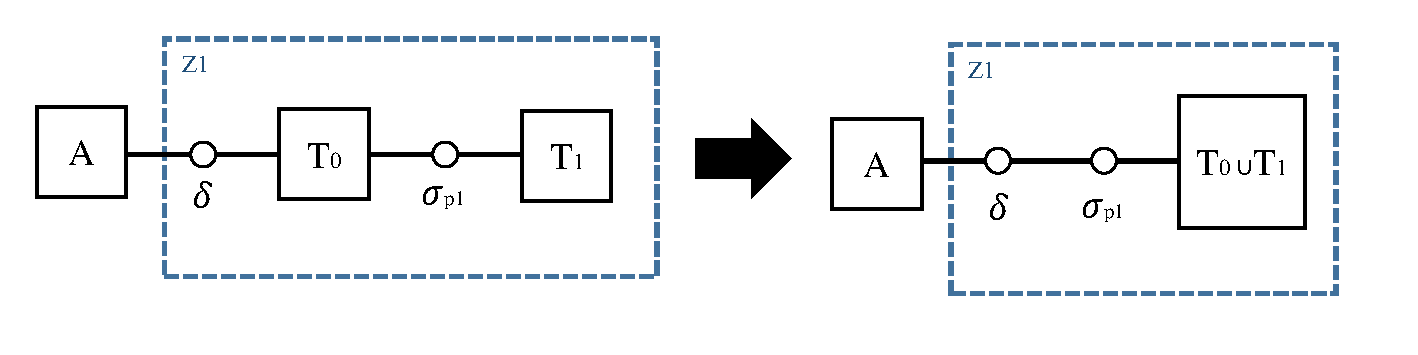
\includegraphics[width=\linewidth]{figures/SQLPatternOptimization} 
	\caption{Horizontal optimization} \label{fig:horizontal_optimization} 
\end{figure} 

\subsection{Horizontal optimization} 

When evaluating a query the normal way (i.e. loading the record set from 
the base table and computing the results), intermediate steps doesn't 
need a materialization. In that case a materialization is only 
reasonable if it pays off over multiple subsequent uses. However, in the 
context of incremental view maintenance, intermediate steps have to be 
materialized. The higher storage cost is traded off against an easy and 
efficient update process -- one base table operation just triggers some 
small view updates. However, not all intermediate steps have to be 
materialized, as this is quite storage consuming. We can already 
optimize a single query by looking at the different zones, depicted in 
Figure~\ref{fig:sql_pattern}. As all the view tables within a zone share 
the same row keys, there is no need of materializing them separately; 
view expression can be combined and the zone just needs one 
materialization (cf. Figure~\ref{fig:horizontal_optimization}). 

So, how can multiple view expressions be combined to affect the 
same materialized view. From a logical point of view, it seems trivial. 
We delete the table nodes, concatenate the operations and build a new 
table node (cf. Figure~\ref{fig:horizontal_optimization}). However, in 
practice we have to make two modifications: (1) the maintenance 
plan has to be updated, (2) the functionality of VMs needs to be 
adapted. 



\noindent
\textbf{Updating the maintenance plan:} To merge the table nodes of a 
zone, we need all expression nodes and table nodes of that zone in a 
sequence. Lets assume, the expression nodes of a zone are defined in 
correct order as $V_{X_{zone}}=\langle v_{x_1},..,v_{x_n}\rangle \subset 
V_X$; the corresponding table nodes of the zone are defined as 
$V_{T_{zone}}=\langle v_{T_1},...,v_{T_n}\rangle \subset V_T$. Further, 
each table node refers to a table with the same row key (this is given 
as long as table nodes are in the same zone). Now, we can update the
zone as depicted by algorithm.


\begin{algorithm}
\caption{Horizontal merging}
\label{alg:assignvm}
\begin{algorithmic}[5]
\Procedure{$horizontalMerge$}{$V_{X_{merge}}, V_{T_{merge}}$}
\ForAll{$v \in V_{T_{merge}}$}
\State $remove(v)$\Comment{queue marker}	
\EndFor
\ForAll{$v \in V_{X_{merge}}$}
\State $remove(outgoingEdges(v))$
\ForAll{$e \in ingoingEdges(v)$}
\State $setTarget(e, lastV)$
\EndFor
\State $lastV \leftarrow v$
\EndFor
\EndProcedure
\end{algorithmic}
\end{algorithm}


\noindent
\textbf{Adapting VMs functionality:} So far, the maintenance plan only 
consists of alternating expression and table nodes. The VM receives a
client operation. It looks up where the client operation comes from. Thus,
it knows the next expression and table node. It simply applies the 
expression and inserts the result into the corresponding table node.
After optimization, multiple expressions can be applied in a row.
Just applying all expressions to the same table is not an option; this
would reduce storage space, but the processing effort would be the
same. Therefore, we also concatenate the execution of the expression. 
To do so, we take a look at execution of the maintenance plan at VM: 


According to Jacobsens 
algorithm a view update algorithm consists of three parts: (1) 
retrieving the old view record, which, in a KV-store architecture, 
conforms to a $get$-operation; (2) computing the new view record, which 
is done locally by a function $compute$ (3) adding the new, or deleting 
the old view record, which conforms to a $put$- or a $delete$-operation. 
If a view table is updated with a single basic view expression, those 
three steps are executed differently depending on the type of view 
expression (i.e. selection, projection, aggregation, etc.). However, if 
we update a view table with multiple view expressions at once, the three 
steps need to be combined. So, if we merge $V_{x_1},..,V_{x_n}$, we 
likewise need to concatenate their get, compute and put functions. 




\begin{equation} 	   
    get(x_1) \circ ... \circ get(x_n)
\end{equation}
\begin{equation} 	   
    compute(x_1) \circ ... \circ compute(x_n)
\end{equation}
\begin{equation} 	   
    put(x_1) \circ ... \circ put(x_n)
\end{equation}




\textit{Example:} Let a base table with a row key $k$ and three columns 
be defined as $A(k, c_1, c_2, c_3)$. Let further a combination of view 
expressions be defined as $\delta$, $\sigma_{c_1 < 10}$ and $\pi_{c_2, 
c_3}$. As soon as a base table operation (let it be an insert or an 
delete operation) is propagated all three steps of the algorithm have to 
be executed for a concatenation of all three expressions. Since Step 1 
is equal for all three expressions we obtain the following equation: 
$get(k) \circ get(k) \circ get(k)=get(k)$. Instead of fetching the same 
record three times, we just fetch it once. Step 1 delivers the old view 
record $r'$. Step 2 computes the new view record, which is different for 
all three operations. Let the client operation be an insert into the 
base table. Then we obtain the following concatenation: $r \circ if(c_1 
< 10)then r; else \emptyset \circ r\\\{c_1\}=if(c_1 < 10)then 
r\\\{c_1\}; else \emptyset$. The delta expression just writes back 
record $r$ such that the old record is available if another operation is 
performed on the same row key. The selection expression writes back the 
record or nothing depending on the selection condition. The projection 
writes back only a selected number of columns. By combining those 
expressions, we derive a new expression, which is shown on the right 
side of the equation. In the last Step 3, we simply write the new record
back to the view, which is similar for all views again: $put(k) \circ 
put(k) \circ put(k)=put(k)$. Instead of three puts, we just perform one.

In this section, we have discussed how multiple view expression in a 
query DAG can be combined to create one materialized view. This 
technique can be regarded as local optimization, as we perform it on
a single query. It reduces the storage capacity needed, as well as the
amount of total update operations in the VMS.




    





